% !TeX program = xelatex
\documentclass[11pt]{article}

% Change "review" to "final" to generate the final (camera-ready) version.
% Change to "preprint" to generate a non-anonymous version with page numbers.
\IfFileExists{acl.sty}{
  \usepackage[preprint]{acl}
}{
  % Fallback when acl.sty is unavailable in local TeX environment.
  \usepackage[a4paper,margin=1in]{geometry}
}

% Standard package includes
\usepackage{iftex}
\usepackage{times}
\usepackage{latexsym}
\usepackage{microtype}
\usepackage{inconsolata}
\usepackage{graphicx}
\usepackage{amsmath}
\usepackage{booktabs}
\usepackage{url}
\usepackage{float}
\usepackage{placeins}
\usepackage{needspace}
\ifXeTeX
  \usepackage{fontspec}
  \usepackage{xeCJK}
  \setmainfont{Times New Roman}
  \setCJKmainfont{SimSun}
\else
  \usepackage[T1]{fontenc}
  \usepackage[utf8]{inputenc}
  \usepackage{CJKutf8}
\fi
\raggedbottom

\title{HW1：从零构建三层 MLP 实现 Fashion-MNIST 分类}

\author{
  洪家权 \\
  \texttt{23307110248@m.fudan.edu.cn}
}

\begin{document}
\ifXeTeX\else\begin{CJK*}{UTF8}{gbsn}\fi
\maketitle

\begin{abstract}
本报告介绍了使用 NumPy 从零实现三层多层感知机（MLP）进行 Fashion-MNIST 分类的过程。项目在不依赖 PyTorch、TensorFlow、JAX 等自动微分框架的前提下，实现了自定义自动微分与反向传播，并完成了训练、验证、超参数搜索和测试评估的完整流程。最终提交模型（\texttt{best\_model\_full}）采用 ReLU 激活函数、隐藏层维度 256、批大小 64、学习率 0.30，并将 L2 正则化系数设为 $\lambda=10^{-4}$；在验证阶段最优模型（\texttt{best\_model\_val}）上取得最佳验证准确率 \texttt{90.52\%}，最终提交模型在测试集上的准确率为 \texttt{89.96\%}，宏平均 F1 为 \texttt{0.899562}。
\end{abstract}

\section{引言}
本报告聚焦于在 Fashion-MNIST 数据集上从零实现三层神经网络分类器，并给出从训练、验证到测试的完整实验流程。当前实现已包含验证集选优、最优权重自动保存、网格搜索与测试集评估。下文将依次介绍模型结构与优化方法，并展示实验结果和可视化分析。

\section{模块设计}
代码主要分为五个部分：数据处理、模型与自动微分、训练优化、超参数搜索和测试评估。数据加载与预处理由 \texttt{dataloader.py} 完成，负责读取 IDX 原始文件、归一化和 one-hot 编码。模型与自动微分由 \texttt{model.py} 实现，包含线性层、激活函数、稳定交叉熵与基于计算图记录（Tape）的自动微分和反向传播。训练与优化由 \texttt{train.py} 实现，包含 mini-batch SGD、学习率衰减、L2 正则、验证集划分、early stopping 和最佳模型保存。超参数搜索由 \texttt{grid\_search.py} 实现，支持多随机种子评估与搜索日志汇总。测试评估由 \texttt{test.py} 实现，输出测试精度、混淆矩阵、第一层权重可视化等数据。

\section{数据与模型}
本实现读取 Fashion-MNIST 的原始 IDX 文件，将每张 $28\times 28$ 灰度图展开为 784 维向量，并将像素归一化到 $[0,1]$。标签被转换为 one-hot 向量以配合交叉熵损失。训练阶段采用分层划分构造验证集（\texttt{val\_ratio=0.2}，\texttt{split\_seed=42}），以保持各类别比例稳定并保证可复现。

本实验实现三层全连接神经网络（输入层 + 单隐藏层 + 输出层），其前向计算为：
\begin{align*}
z_1 &= XW_1 + b_1, \\
a_1 &= \phi(z_1), \\
z_2 &= a_1W_2 + b_2 .
\end{align*}
其中 $\phi(\cdot)$ 可在 ReLU 与 Sigmoid 之间切换，隐藏层维度可配置，输出层固定为 10 类。激活函数通过训练配置在 ReLU 与 Sigmoid 之间切换；当使用 ReLU 时配套 He 初始化，使用 Sigmoid 时配套 Xavier 初始化。

\section{自动微分与反向传播}
项目实现了基于计算图记录（Tape）的自动微分机制。前向传播时，每个算子记录输入、输出和局部梯度函数；反向传播时按逆序回放计算图并累加梯度。线性层、激活函数和 softmax 交叉熵都提供了解析梯度，因此能够在纯 NumPy 环境下完成端到端反向传播。

对三层 MLP，参与梯度回传的参数节点为 $\{W_1,b_1,W_2,b_2\}$，中间节点为 $\{z_1,a_1,z_2\}$。反向链路可写为
\[
\begin{aligned}
\frac{\partial \mathcal{L}_{ce}}{\partial z_2}
&\rightarrow
\left(
\frac{\partial \mathcal{L}_{ce}}{\partial W_2},
\frac{\partial \mathcal{L}_{ce}}{\partial b_2},
\frac{\partial \mathcal{L}_{ce}}{\partial a_1}
\right)\\
&\rightarrow
\frac{\partial \mathcal{L}_{ce}}{\partial z_1}
\rightarrow
\left(
\frac{\partial \mathcal{L}_{ce}}{\partial W_1},
\frac{\partial \mathcal{L}_{ce}}{\partial b_1}
\right).
\end{aligned}
\]
其中激活函数梯度由局部导数显式接入：ReLU 使用 $\mathbf{1}(z_1>0)$，Sigmoid 使用 $\sigma(z_1)(1-\sigma(z_1))$。因此无论选择 ReLU 还是 Sigmoid，链式法则将输出层损失梯度正确传递到第一层参数。

交叉熵采用数值稳定的 log-sum-exp 形式。设 logits 为 $z$，one-hot 标签为 $y$：
\begin{equation*}
\mathcal{L}_{ce}=-\frac{1}{N}\sum_{i=1}^{N}\sum_{c=1}^{C}y_{ic}\log p_{ic},\quad p=\mathrm{softmax}(z),
\end{equation*}
其中，$N$ 为 batch 样本数，$C$ 为类别数，$y_{ic}$ 为样本 $i$ 在类别 $c$ 的 one-hot 标签，$p_{ic}$ 为对应预测概率。则对 logits 的梯度为：
\begin{equation*}
\frac{\partial \mathcal{L}_{ce}}{\partial z}=\frac{p-y}{N}.
\end{equation*}
为验证实现正确性，代码还提供了数值梯度检查脚本，对有限差分梯度与解析梯度进行对比。
在 ReLU 设置下，我们采用中心差分对 $W_1/b_1/W_2/b_2$ 各随机采样 8 个参数点进行校验。终端汇总结果为
$\mathrm{max\_rel\_err}=3.047102\times10^{-11}$、
$\mathrm{mean\_rel\_err}=1.152229\times10^{-11}$，
最终判定为 PASS。相对误差量级低至 $10^{-11}$，表明解析梯度与数值梯度高度吻合。

此外，脚本支持将详细校验结果写入 JSON 文件（包含运行设置、$W_1/b_1/W_2/b_2$ 的随机抽样索引、每个采样点的 $g_{num}/g_{ana}/rel\_err$ 以及最终 PASS/FAIL 汇总），便于复核与复现实验。对应结果文件为 \path{ExtraData/grad_check_result.json}。
上述数值检验在固定超参与随机种子下对参数子集抽样进行，验证该条件下解析梯度与反传实现同有限差分的一致性。

\section{训练与超参数搜索}
训练目标由交叉熵与 L2 正则共同组成：
\begin{equation*}
\mathcal{L}_{total}=\mathcal{L}_{ce}+\frac{\lambda}{2}\left(\|W_1\|_2^2+\|W_2\|_2^2\right).
\end{equation*}
在实现中，反向传播先由 Tape 计算 $\nabla \mathcal{L}_{ce}$，再在参数梯度上并入正则项，即
\[
\begin{aligned}
\nabla_{W_1}\mathcal{L}_{total}
&=\nabla_{W_1}\mathcal{L}_{ce}+\lambda W_1,\\
\nabla_{W_2}\mathcal{L}_{total}
&=\nabla_{W_2}\mathcal{L}_{ce}+\lambda W_2.
\end{aligned}
\]
偏置项 $b_1,b_2$ 不加入 L2 惩罚。
优化器采用 mini-batch SGD：
\begin{equation*}
\theta_{k+1}
=\theta_k-\eta_k\cdot \frac{1}{|B_k|}
\sum_{(x_i,y_i)\in B_k}\nabla_{\theta}\mathcal{L}(x_i,y_i;\theta_k).
\end{equation*}
其中，$\theta_k$ 表示第 $k$ 次迭代的参数集合（含 $W_1,b_1,W_2,b_2$），$B_k$ 为该次迭代使用的 mini-batch，$|B_k|$ 为 batch 大小，$\eta_k$ 为当前步学习率，$\mathcal{L}$ 为单样本训练目标（交叉熵与 L2 正则之和）。
学习率使用余弦衰减：
\begin{equation*}
\eta_t=\eta_{\max}\cdot\frac{1+\cos(\pi t/(T-1))}{2}.
\end{equation*}
其中 $t$ 为 epoch 索引（从 0 开始），$T$ 取总训练轮数 \texttt{epochs}；即每个 epoch 更新一次学习率，并在整个训练过程中持续生效。
训练过程中包含全局梯度裁剪、数值稳定性监测及损失、梯度与参数的异常检测，并采用与激活函数匹配的参数初始化。本文最终实验设置为：\texttt{epochs=50}、\texttt{patience=7}、\texttt{min\_delta}=$10^{-4}$、\texttt{grad\_clip\_norm=1.0}。
梯度裁剪采用全局范数约束：先对 $\{dW_1,db_1,dW_2,db_2\}$ 的平方和开方得到全局梯度范数，若超过 \texttt{grad\_clip\_norm=1.0}，则按统一比例缩放全部梯度；否则保持不变。

验证阶段在每个训练轮次结束时于验证集评估性能。若验证准确率相对历史最优的提升超过预设容差，则更新检查点；若二者差距落在该容差带宽内而视为平局，则保留验证总损失更小者。连续若干轮未触发上述改进条件则早停。检查点按轮次粒度保存，内容为全部网络权重及所用激活函数。
完成超参数确定后，在训练与验证样本合并得到的完整训练集上重新训练，并以所得模型作为测试集评估与报告结论的依据；验证阶段保留的检查点仅用于超参数遴选及与训练过程的对照分析。

超参数搜索采用网格搜索，覆盖学习率、隐藏层大小、batch size、L2 强度与激活函数组合，并支持多随机种子统计均值后选优。

\section{实验结果}
\subsection{六轮网格搜索范围}
\begin{table}[H]
\centering
\resizebox{\linewidth}{!}{
\begin{tabular}{clcccc}
\toprule
轮次ID & 学习率搜索区间 & 隐藏层 & Batch & $\lambda$（L2） & 激活函数 \\
\midrule
R1 & \{0.005, 0.01, 0.05\} & \{128, 256\} & \{64, 128\} & \{$10^{-4}$, $10^{-3}$\} & \{relu, sigmoid\} \\
R2 & \{0.05, 0.07, 0.09, 0.10\} & \{128, 256\} & \{64\} & \{$10^{-4}$, $10^{-3}$\} & \{relu\} \\
R3 & \{0.08, 0.09, 0.10, 0.11, 0.12, 0.14, 0.15\} & \{256\} & \{64\} & \{$10^{-4}$\} & \{relu\} \\
R4 & \{0.14, 0.15, 0.16, 0.18, 0.20\} & \{256\} & \{64\} & \{$10^{-4}$\} & \{relu\} \\
R5 & \{0.18, 0.20, 0.22, 0.24, 0.25\} & \{256\} & \{64\} & \{$10^{-4}$\} & \{relu\} \\
R6 & \{0.24, 0.25, 0.26, 0.28, 0.30\} & \{256\} & \{64\} & \{$10^{-4}$\} & \{relu\} \\
\bottomrule
\end{tabular}
}
\caption{各轮网格搜索范围（由搜索日志提取）。}
\label{tab:grid-ranges}
\end{table}

由表1可见，搜索过程从第 1 轮的宽范围粗搜索逐步收敛到第 6 轮的高学习率细化区间，其间隐藏层、批大小、激活函数与正则化设置逐步固定，体现了“先粗后细”的搜索策略。

\subsection{六轮搜索结果}
\begin{table}[H]
\centering
\resizebox{\linewidth}{!}{
\begin{tabular}{ccccc}
\toprule
轮次ID & 最优学习率 & 验证集均值准确率 & 测试集准确率 & 最佳验证轮次 \\
\midrule
R1 & 0.05 & 0.8747 & 88.35\% & 41 \\
R2 & 0.10 & 0.8887 & 89.42\% & 21 \\
R3 & 0.15 & 0.8946 & 90.07\% & 35 \\
R4 & 0.20 & 0.8973 & 89.99\% & 40 \\
R5 & 0.25 & 0.8989 & 89.98\% & 45 \\
R6 & 0.30 & 0.8992 & 89.96\% & 47 \\
\bottomrule
\end{tabular}
}
\caption{六轮实验汇总：最优学习率、验证集均值准确率、测试集准确率与最佳验证 epoch。其中，\texttt{R1--R6} 分别对应第 1--6 轮调参（\texttt{TuningRound1--TuningRound6}）。}
\label{tab:round-summary}
\end{table}

由表2可见，第 1 轮调参（\texttt{TuningRound1}）到第 6 轮调参（\texttt{TuningRound6}）的最优结果显示：最优配置逐步收敛到隐藏层维度 256、批大小 64、ReLU 激活函数和 L2 正则化系数 $10^{-4}$，最佳学习率从 0.05 提升至 0.30，验证集均值准确率稳步上升，但后期提升幅度变小。

本报告选择 \texttt{TuningRound6} 的结果作为最终搜索结果，原因是其在六轮候选中具有最高的验证集均值准确率（\texttt{best\_val\_acc\_mean}）。训练阶段的 \texttt{BestEpoch} 判定规则为：优先最大化 \texttt{val\_acc}；当 \texttt{val\_acc} 在 \texttt{min\_delta} 范围内并列时，采用更低的 \texttt{val\_total\_loss}（交叉熵+L2）作为平局决断依据；若连续 \texttt{patience} 轮无提升则触发早停。该步骤输出的是验证阶段最优模型 \texttt{best\_model\_val}；正文后续报告的测试集指标来自对应超参数下全量重训得到的 \texttt{best\_model\_full}。

由后续第九部分的混淆矩阵统计可见，测试准确率整体约为 90\%，后几轮验证指标继续提升而测试指标基本稳定，说明模型在高学习率区间的泛化能力已趋于饱和。

\subsection{最终轮稳定性与收敛轮次}
\begin{table}[H]
\centering
\small
\setlength{\tabcolsep}{4pt}
\resizebox{\linewidth}{!}{
\begin{tabular}{lccc}
\toprule
ID & Val Acc Mean & Val Acc Std & Best Seed Acc \\
\midrule
S1 & 0.8984 & 0.0015 & 0.9006 \\
S2 & 0.8989 & 0.0011 & 0.9004 \\
S3 & 0.8988 & 0.0015 & 0.9005 \\
S4 & 0.8986 & 0.0009 & 0.8998 \\
S5 & \textbf{0.8992} & 0.0013 & \textbf{0.9014} \\
\bottomrule
\end{tabular}
}
\normalsize
\caption{最终轮多种子稳定性。其中，\texttt{S1--S5} 分别对应学习率 \texttt{0.24, 0.25, 0.26, 0.28, 0.30}（其余设置一致：隐藏层维度为 256、批大小为 64、激活函数为 ReLU，且 L2 正则化系数为 $10^{-4}$）。}
\label{tab:round6-stability}
\end{table}

由表3可知，最终采用的 \texttt{S5} 配置在本轮候选中取得最高的验证集均值准确率（\texttt{Val Acc Mean=0.8992}）与最高单种子准确率（\texttt{Best Seed Acc=0.9014}），体现了其最优性。同时，\texttt{S5} 的跨种子波动为 \texttt{Val Acc Std=0.0013}，且对应最佳 epoch 集中在 \texttt{14--18}（均值约 \texttt{15.8}），说明该配置在精度水平与收敛稳定性之间保持了较好平衡。

从 \texttt{TuningRound6} 整体看，\texttt{S1--S5} 的准确率均值、准确率标准差与最佳种子准确率均表现为小幅波动：\texttt{Val Acc Mean} 位于 \texttt{0.8984--0.8992}，\texttt{Val Acc Std} 位于 \texttt{0.0009--0.0015}，\texttt{Best Seed Acc} 位于 \texttt{0.8998--0.9014}。三项指标均未随学习率单调递增，而是在窄区间内上下波动，说明在该高学习率细化区间继续提高学习率的边际效益已不足。综合最优性能与稳定性，本报告最终选择 \texttt{S5}（学习率 \texttt{0.30}）作为后续全量训练与测试评估的配置。
\FloatBarrier
\Needspace{16\baselineskip}
\subsection{消融实验与效率-性能权衡}
\begin{table}[H]
\centering
\small
\setlength{\tabcolsep}{4pt}
\resizebox{\linewidth}{!}{
\begin{tabular}{lccc}
\toprule
ID & Val Acc Mean & $\Delta$ vs Baseline & Elapsed Sec \\
\midrule
A0 & \textbf{0.8747} & -- & 1039.62 \\
A1 & 0.8459 & -0.0289 & 1003.25 \\
A2 & 0.8739 & -0.0008 & 562.91 \\
A3 & 0.8673 & -0.0074 & 561.66 \\
A4 & 0.8734 & -0.0014 & 1056.09 \\
\bottomrule
\end{tabular}
}
\normalsize
\caption{基于第 1 轮调参（\texttt{TuningRound1}）搜索日志的消融与效率对比。其中，\texttt{A0} 为基线设置（激活函数为 ReLU、隐藏层维度为 256、批大小为 64、L2 正则化系数为 $10^{-4}$）；\texttt{A1} 仅将激活函数改为 Sigmoid；\texttt{A2} 仅将隐藏层维度改为 128；\texttt{A3} 仅将批大小改为 128；\texttt{A4} 仅将 L2 正则化系数改为 $10^{-3}$。}
\label{tab:ablation-round1}
\end{table}

由表4可见，在统一搜索框架下，对比可见：激活函数带来的性能差异最显著（ReLU 明显优于 Sigmoid）；增大隐藏层维度仅带来有限收益但训练耗时显著增加；较大的 batch 在当前设置下精度下降；过强的 L2（$\lambda=10^{-3}$）略抑制性能。实验表明，本任务中性能主要受激活函数与学习率区间主导，结构增大并非同等性价比的提升路径。

\FloatBarrier
\Needspace{12\baselineskip}
\section{训练曲线可视化}

从本节开始统一约定：\texttt{best\_model\_val} 表示验证阶段最优模型（用于选参与曲线展示），\texttt{best\_model\_full} 表示固定超参数后在 \texttt{train+val} 上重训得到的最终提交模型（用于测试、混淆矩阵与错例分析）。

\begin{figure}[htbp]
\centering

\includegraphics[width=0.95\linewidth]{../TuningRound6/figures/history.png}
\caption{Figure1:\texttt{best\_model\_val} 对应训练过程的学习曲线。左图为训练/验证损失（含 total 与 ce），右图为训练/验证准确率；其中验证集准确率用于模型选优。}
\label{fig:history}
\end{figure}

图 \ref{fig:history} 展示了 \texttt{best\_model\_val} 对应训练过程在验证集划分阶段的收敛轨迹。训练早期，\texttt{train\_total\_loss} 与 \texttt{val\_total\_loss} 同步快速下降，\texttt{val\_acc} 快速上升；进入中后期后，损失曲线下降趋缓、准确率进入平台区，表现出与余弦学习率衰减和 mini-batch SGD 一致的“先快后稳”优化轨迹。
从量化结果看，\texttt{train\_total\_loss} 由 0.4695 下降到 0.1486（约下降 68.4\%），\texttt{val\_total\_loss} 由 0.4819 下降到 0.3419（约下降 29.1\%）；\texttt{train\_acc} 从 0.8386 提升到 0.9706，\texttt{val\_acc} 从 0.8333 提升到 0.9050。该图同时给出 \texttt{train\_ce\_loss} 与 \texttt{val\_ce\_loss}，用于与 total loss（交叉熵+L2）对照观察，验证训练过程稳定并支撑基于验证集指标的模型选优。

\FloatBarrier
\Needspace{12\baselineskip}
\section{第一层权重可视化与空间模式}
\begin{figure}[htbp]
\centering

\includegraphics[width=\linewidth]{../TuningRound6/figures/weight1_grid.png}
\caption{第一层隐藏层权重可视化（最终模型）。}
\label{fig:w1-grid}
\end{figure}

图 \ref{fig:w1-grid} 将第一层参数矩阵 $W_1\in\mathrm{R}^{784\times H}$ 的列向量重排为 $28\times 28$ 模板，并展示范数较大的前 32 个神经元。归一化后，这些图像可视为空间敏感区域的相对分布：亮度变化越明显，表示该神经元在对应区域学习到更强判别模式。
本节展示的是训练后权重。由于未并列展示随机初始化权重对照图，因此这里主要说明训练后权重中出现了可解释的空间模板；该结果不足以直接证明训练前后差异的变化过程。

从空间结构看，第一层主要学到四类模板：第一类为近中心纵向条带与对称轴响应，可编码上装/下装主体轮廓；第二类为上半区弧形与斜向边缘，对应领口、肩线和袖口过渡；第三类为下半区水平边界与块状响应，对应衣摆、裙摆或裤脚终止位置；第四类为背景-前景过渡模板（四角与边界区域），用于抑制背景噪声并突出主体形状。其共性是关注轮廓特征而非纹理细节。

结合后续混淆矩阵可进一步解释其作用边界：对轮廓差异明显的类别，上述模板通常足够区分；但对局部细节更关键的相近上装类别，仅依赖第一层形状模板仍会出现重叠响应，造成系统性混淆。从更高层面看，第一层权重可视化与混淆结构共同说明：模型在全局外形上已学到较一致的线索，而在依赖局部差异的类别边界上仍容易犹豫；Top-K 混淆长期集中在上装内部，是这一现象在统计上的体现。

上装子类间的混淆，除与第一层更偏轮廓的响应有关外，也与网络较浅、展平后全连接的设定有关。在此设定下，像素邻域仅靠全连接权重隐式拟合，缺少卷积等结构中的局部与共享归纳偏置，对领口、袖长等部件级差异的区分仍相对吃力。若要进一步压低此类错误，可能需要更深或带图像先验的网络结构。

\FloatBarrier
\Needspace{12\baselineskip}
\section{混淆矩阵分析}
\subsection{混淆矩阵可视化}
\FloatBarrier
\begin{figure}[H]
\centering

\includegraphics[width=0.82\linewidth]{../TuningRound6/figures/confusion_count.png}
\caption{测试集混淆矩阵（计数，最终模型）。}
\label{fig:cm}
\end{figure}
\FloatBarrier

图 \ref{fig:cm} 给出了测试集混淆矩阵。整体上，轮廓差异明显的类别（如 Trouser、Bag、Sneaker）识别较稳定；而外观相近的上装类别（T-shirt/top、Shirt、Pullover、Coat）仍存在较多混淆。这与低分辨率灰度图中纹理与细粒度语义不足的特点一致。
本文主文展示计数混淆矩阵；按行归一化（召回率视角）的信息由表 \ref{tab:per-class-prf} 的各类 Recall 指标补充呈现，用于避免样本规模对计数直观比较的干扰。

\subsection{Top-K 混淆对定量统计}
根据 9.1 中的混淆矩阵图，最终模型在测试集共 10000 张样本，其中正确 8996、错误 1004。按“双向类别对”聚合后，前 6 大混淆对分别为
\texttt{T-shirt/top $\leftrightarrow$ Shirt (197)}、
\texttt{Pullover $\leftrightarrow$ Coat (163)}、
\texttt{Pullover $\leftrightarrow$ Shirt (144)}、
\texttt{Coat $\leftrightarrow$ Shirt (106)}、
\texttt{Dress $\leftrightarrow$ Coat (57)}、
\texttt{Sneaker $\leftrightarrow$ Ankle boot (57)}，
合计 724 次，占全部错误约 72.1\%。这说明错误主要集中在少数语义/轮廓相近类别之间，而非均匀分布。

\FloatBarrier
\begin{table}[H]
\centering
\begin{tabular}{lc}
\toprule
Confused Pair (bidirectional) & Error Count \\
\midrule
T-shirt/top $\leftrightarrow$ Shirt & 197 \\
Pullover $\leftrightarrow$ Coat & 163 \\
Pullover $\leftrightarrow$ Shirt & 144 \\
Coat $\leftrightarrow$ Shirt & 106 \\
Dress $\leftrightarrow$ Coat & 57 \\
Sneaker $\leftrightarrow$ Ankle boot & 57 \\
\bottomrule
\end{tabular}
\caption{测试集 Top-6 混淆类别对（基于计数混淆矩阵双向合并）。}
\label{tab:top-confused-pairs}
\end{table}
\FloatBarrier

\subsection{高置信错分现象}
根据 \texttt{error\_cases.csv} 的前 10 个高置信错例，预测置信度均高于 0.998，表明模型在少量难例上会出现置信度较高但预测错误的情况。这些错例主要集中在上装细分类别与鞋类边界类别之间，说明模型存在明确的错分模式，而不是随机引入的误差。
需要指出，当前错例分析是基于代表性个案进行错分模式分析。

\subsection{每类指标（Precision / Recall / F1）}
基于 \texttt{confusion\_matrix.csv} 计算每类指标如下。

\begin{table}[H]
\centering
\small
\setlength{\tabcolsep}{4pt}
\begin{tabular}{lccc}
\toprule
ID & Precision & Recall & F1 \\
\midrule
C0 & 0.8615 & 0.8520 & 0.8567 \\
C1 & 0.9929 & 0.9800 & 0.9864 \\
C2 & 0.8060 & 0.8270 & 0.8164 \\
C3 & 0.9020 & 0.9110 & 0.9065 \\
C4 & 0.8231 & 0.8420 & 0.8324 \\
C5 & 0.9797 & 0.9630 & 0.9713 \\
C6 & 0.7516 & 0.7260 & 0.7386 \\
C7 & 0.9443 & 0.9660 & 0.9550 \\
C8 & 0.9749 & 0.9710 & 0.9729 \\
C9 & 0.9609 & 0.9580 & 0.9594 \\
\bottomrule
\end{tabular}
\normalsize
\caption{测试集每类 Precision / Recall / F1（最终模型）。其中，\texttt{C0--C9} 分别对应 \texttt{T-shirt/top, Trouser, Pullover, Dress, Coat, Sandal, Shirt, Sneaker, Bag, Ankle boot}。}
\label{tab:per-class-prf}
\end{table}
从表 \ref{tab:per-class-prf} 可见，总体准确率为 \texttt{89.96\%}，宏平均精确率为 \texttt{89.97\%}，宏平均召回率为 \texttt{89.96\%}，宏平均 F1 为 \texttt{0.899562}，说明类别不均衡影响较小。类别层面上，\texttt{Shirt} 的 F1 最低（0.7386），与其在上装子类中的高混淆现象一致；\texttt{Trouser}、\texttt{Sandal}、\texttt{Bag}、\texttt{Ankle boot} 指标较高，说明这些类别的轮廓判别性更强。

\FloatBarrier
\Needspace{14\baselineskip}
\section{错例分析}
\subsection{误差集中度与类别难度}
测试集共 10000 张样本，其中错误 1004 张（10.04\%）。错误并非均匀分布，而是集中在少数语义相近类别。以双向类别对统计，前 6 组混淆合计 724 次，占全部错误的 72.1\%。进一步聚焦上装子类（\texttt{T-shirt/top, Pullover, Coat, Shirt}），其内部两两混淆合计 648 次，占全部错误的 64.5\%，说明主要瓶颈来自细粒度上装边界，而非全局识别失败。

从每类错误率（$1-\mathrm{Recall}$）来看，\texttt{Shirt}（27.4\%）、\texttt{Pullover}（17.3\%）、\texttt{Coat}（15.8\%）和 \texttt{T-shirt/top}（14.8\%）的分类难度相对更高；而 \texttt{Trouser}（2.0\%）、\texttt{Bag}（2.9\%）和 \texttt{Sneaker}（3.4\%）错误率较低。这表明，轮廓明显的类别相较于轮廓模糊的，更容易被MLP正确区分。

\subsection{方向性混淆与边界偏置}
除双向统计外，方向性统计可用于刻画类别边界是否存在单向吸附。定义方向不对称系数为
\[
A_{i,j}=\frac{|M_{i,j}-M_{j,i}|}{M_{i,j}+M_{j,i}},
\]
其中 $M_{i,j}$ 表示真实类别 $i$ 被预测为类别 $j$ 的次数。该系数满足 $A\in[0,1]$：当 $A\approx0$ 时，说明两方向错分规模接近，边界近似对称；当 $A$ 较大时，说明某一方向明显更多，存在方向偏置。该指标可作为后续误差归因与模型改进（如类间重加权、细粒度特征增强）的定量依据，也便于区分结构性偏差与偶发噪声错误。

\subsection{高置信错例分类型分析}
根据 \texttt{error\_cases.csv} 的前 10 个高置信错例，置信度范围为 $[0.9983,\,0.9999]$，均值约为 $0.9992$，表明错误并非低置信随机波动，而是模型在少量难例上形成了稳定但错误的高置信决策，且具有可重复的模式特征。结合语义结构与方向不对称系数，本文将错例归纳为上装混淆、鞋类混淆与跨语义类别混淆三类。

\subsubsection{上装混淆}
\begin{figure}[H]
\centering

\includegraphics[width=0.5\linewidth]{../TuningRound6/figures/errors/err_324_t4_p6.png}\hfill

\includegraphics[width=0.5\linewidth]{../TuningRound6/figures/errors/err_3370_t2_p4.png}\\[0.5em]

\includegraphics[width=0.5\linewidth]{../TuningRound6/figures/errors/err_8373_t6_p2.png}\hfill

\includegraphics[width=0.5\linewidth]{../TuningRound6/figures/errors/err_5806_t6_p0.png}
\caption{上装混淆错例：(a) Coat$\rightarrow$Shirt，(b) Pullover$\rightarrow$Coat，(c) Shirt$\rightarrow$Pullover，(d) Shirt$\rightarrow$T-shirt/top。}
\label{fig:error-cases-upper}
\end{figure}

图\ref{fig:error-cases-upper}中的示例图片对应 \texttt{error\_cases.csv} 前五中的第 1、2、3、5 条。这些样本在领口、袖口与衣长等局部线索上较模糊，模型更依赖整体轮廓。结合方向系数可见，不同上装对的对称性存在差异：\texttt{Pullover$\leftrightarrow$Coat} 的 $A\approx0.018$、\texttt{Shirt$\leftrightarrow$T-shirt/top} 的 $A\approx0.025$，均接近对称；而 \texttt{Shirt$\leftrightarrow$Pullover} 的 $A\approx0.125$，方向偏置更明显，说明该边界更容易出现单向吸附。

\subsubsection{鞋类混淆}
\begin{figure}[H]
\centering

\includegraphics[width=0.70\linewidth]{../TuningRound6/figures/errors/err_23_t9_p5.png}
\caption{鞋类混淆错例：Ankle boot$\rightarrow$Sandal。}
\label{fig:error-cases-shoes}
\end{figure}

图\ref{fig:error-cases-shoes}中的示例图片对应 \texttt{error\_cases.csv} 前五中的第 4 条。该样本中鞋帮与鞋口边界不清，局部开口形态更接近凉鞋。对应鞋类对子 \texttt{Sandal$\leftrightarrow$Ankle boot} 的方向系数为 $A\approx0.478$，明显高于上装主混淆对，说明该类别对具有更强方向偏置：模型更倾向将部分踝靴样本误判为凉鞋，而非反向等量错分。

\subsubsection{跨语义类别混淆}
\begin{figure}[H]
\centering
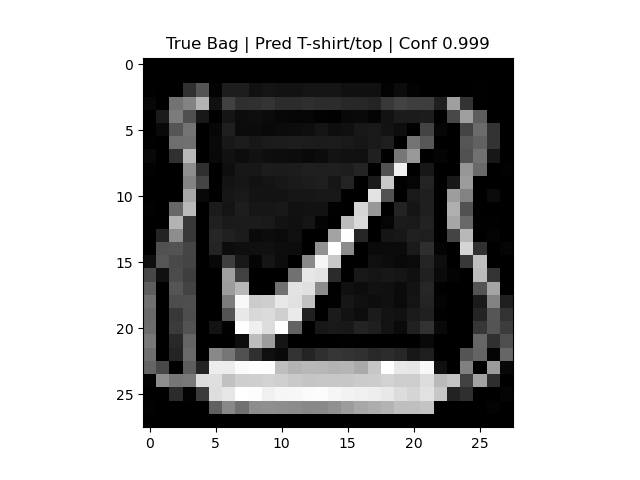
\includegraphics[width=0.5\linewidth]{../TuningRound6/figures/errors/err_669_t8_p0.png}\hfill

\includegraphics[width=0.5\linewidth]{../TuningRound6/figures/errors/err_787_t1_p3.png}
\caption{跨语义类别高置信错例：(a) Bag$\rightarrow$T-shirt/top，(b) Trouser$\rightarrow$Dress。}
\label{fig:error-cases-cross}
\end{figure}

除上述两类主模式外，前 10 个高置信错例中还出现少量跨语义混淆。对应方向系数分别约为 $A\approx0.077$ 与 $A\approx0.412$，前者近似对称、后者方向偏置较强。该现象提示：在少量轮廓极端简化样本上，模型可能优先依赖粗粒度几何形状而忽略语义细节，从而跨类误判。

总体而言，三类错例共同指向同一成因：在低分辨率灰度输入下，模型对全局轮廓线索利用充分，但对区分类别所需的局部细节线索利用不足；这一点与混淆矩阵的集中错分模式及方向不对称统计结果一致。

\section{结论}
本作业完成了从零实现三层 MLP 的完整流程，包括自动微分、反向传播、网格搜索、验证集选优与测试评估。其中，\texttt{best\_model\_val} 用于验证阶段模型选择，\texttt{best\_model\_full} 用于最终测试与提交。最终提交模型采用 ReLU 激活函数、隐藏层维度 256、批大小 64、学习率 0.30，并将 L2 正则化系数设为 $\lambda=10^{-4}$；在验证阶段最优模型上取得最佳验证准确率 \texttt{90.52\%}，最终提交模型在测试集上的准确率为 \texttt{89.96\%}，宏平均 F1 为 \texttt{0.899562}。实验表明：激活函数与学习率区间是最主要影响因素，隐藏层增大带来的收益有限且伴随更高训练开销。模型优势在于训练稳定、可复现且对明显轮廓类别识别较好；局限在于低分辨率灰度输入下对局部细节线索利用不足，导致以上装细粒度类别为主的系统性混淆，并伴随少量鞋类与跨语义类别的高置信错分。

\appendix
\section{附录：代码仓库与模型权重}
\begingroup
\raggedright
\sloppy

\subsection{代码仓库}
\noindent\url{https://github.com/Jacky23307110248/CS50028-ComputerVision}

\vspace{0.35em}
\noindent 本作业（HW1）位于该仓库根目录下的 \texttt{HW1/} 子目录。环境依赖及训练、测试命令见 \texttt{HW1} 子目录下的 \texttt{README.md}，请注意与仓库根目录的 \texttt{README.md} 相区分。

\subsection{模型权重}
\noindent 正文测试集结果与相关图表均来自全量数据重训后的\textbf{最终模型}；其权重相对仓库根路径为：\par
\noindent\url{HW1/TuningRound6/artifacts/best_model_full.npy}

\endgroup

\ifXeTeX\else\end{CJK*}\fi
\end{document}
